\documentclass{article}

\usepackage[utf8]{inputenc}
\usepackage[spanish]{babel}
\usepackage{enumerate}
\usepackage{physics}
\usepackage{amssymb}
\usepackage{graphicx}

\title{Mecánica Cuántica Avanzada\\ Examen Final}
\author{Iván Mauricio Burbano Aldana}

\begin{document}

\maketitle

\begin{enumerate}[1)]

\item

\begin{enumerate}[a)]

\item En el sistema no perturbado cada nivel de energía es generado por un estado descrito por $\psi_n\in L^2([0,L])$ con
\begin{equation}
\psi_n(x)\propto\sin(\frac{n\pi}{L}x)
\end{equation}
para cada $n\in\mathbb{N}^*$. El cálculo
\begin{align}
\begin{split}
\int_0^L\dd{x}\sin(\frac{n\pi}{L}x)^2=&\int_0^L\dd{x}\frac{1-\cos(\frac{2n\pi}{L}x)}{2}\\
=&\frac{L}{2}-\frac{1}{2}\int_0^L\dd{x}\cos(\frac{2n\pi}{L}x)=\frac{L}{2},
\end{split}
\end{align}
donde la integral sobre el coseno desvanece al realizarse sobre un número entero de periodos, muestra que una normalización apropiada para los vectores de estado es
\begin{equation}
\psi_n(x):=\sqrt{\frac{2}{L}}\sin(\frac{n\pi}{L}x).
\end{equation}
La ecuación de valores propios del Hamiltoniano
\begin{align}
\begin{split}
E_n\psi_n(x)=&H\psi_n(x)=-\frac{\hbar^2}{2m}\psi_n''(x)=\frac{\hbar^2}{2m}\qty(\frac{n\pi}{L})^2\sqrt{\frac{2}{L}}\sin(\frac{n\pi}{L}x)\\
=&\frac{\hbar^2\pi^2n^2}{2mL^2}\psi_n(x),
\end{split}
\end{align}
muestra que la energía del estado descrito por $\psi_n$ es
\begin{equation}
E_n:=\frac{\hbar^2\pi^2n^2}{2mL^2}.
\end{equation}

La perturbación al sistema se puede modelar añadiéndole al Hamiltoniano el término $V_0\chi_{[0,L/2]}$, donde 
\begin{equation}
\chi_A(x):=\begin{cases}
1 & x\in A\\
0 & x\not\in A
\end{cases}
\end{equation} 
es la función característica del conjunto $A$. La primera corrección a la energía se puede encontrar como
\begin{align}
\begin{split}
E_n^{(1)}=&\langle\psi_n,V_0\chi_{[0,L/2]}\psi_n\rangle=\frac{2V_0}{L}\int_0^L\dd{x}\chi_{[0,L/2]}(x)\sin(\frac{n\pi}{L}x)^2\\
=&\frac{2V_0}{L}\int_0^{L/2}\dd{x}\sin(\frac{n\pi}{L}x)^2=\frac{2V_0}{L}\int_0^{L/2}\dd{x}\frac{1-\cos(\frac{2n\pi}{L}x)}{2}\\
=&\frac{V_0}{2}-\frac{V_0}{L}\int_0^{L/2}\dd{x}\cos(\frac{2n\pi}{L}x)\\
=&\frac{V_0}{2}-\frac{V_0}{L}\frac{L}{2n\pi}\qty[\sin(\frac{2n\pi}{L}x)]_0^{L/2}=\frac{V_0}{2}.
\end{split}
\end{align}

\item Ya que la perturbación es pequeña no nos interesaremos por describir estados cuya energía es menor. Nos limitamos a notar que en tal caso las soluciones van a ser las de un pozo de longitud $L/2$ en vista de que el método WKB no detecta la altura de las paredes. Asumiendo que queremos describir estados de energía mayores a $V_0$ los puntos de retorno clásicos son $0$ y $L$. Ya que en estos puntos hay paredes rígidas, las energías $E_n$ satisfacen para $n\in\mathbb{N}^*$ la condición de cuantización
\begin{align}
\begin{split}
n\pi\hbar=&\int_0^L\dd{x}p(x)=\int_0^{L/2}\dd{x}\sqrt{2m(E_n-V_0)}+\int_0^{L/2}\dd{x}\sqrt{2mE_n}\\
=&\qty(\sqrt{2m(E_n-V_0)}+\sqrt{2mE})\frac{L}{2}.
\end{split}
\end{align}
Las soluciones de esta ecuación algebraica son
\begin{align}
\begin{split}
\frac{2\hbar\pi n}{L}=&\sqrt{2m(E_n-V_0)}+\sqrt{2mE_n}\\
\frac{4\hbar^2\pi^2 n^2}{L^2}=&2m(E_n-V_0)+2mE_n+4m\sqrt{E_n(E_n-V_0)}\\
2\sqrt{E_n^2-E_nV_0}=&\frac{2\hbar^2\pi^2 n^2}{mL^2}-2E_n+V_0\\
4E_n^2-4E_nV_0=&4E_n^2+\qty(\frac{2\hbar^2\pi^2 n^2}{mL^2}+V_0)^2-4E_n\qty(\frac{2\hbar^2\pi^2 n^2}{mL^2}+V_0)\\
4E_n\frac{2\hbar^2\pi^2 n^2}{mL^2}=&\qty(\frac{2\hbar^2\pi^2 n^2}{mL^2}+V_0)^2\\
E_n=&\frac{m}{2}\frac{\qty(\frac{2\hbar^2\pi^2 n^2}{mL^2}+V_0)^2}{\qty(\frac{2\hbar\pi n}{L})^2}=\frac{m}{2}\qty(\frac{\hbar\pi n}{mL}+\frac{LV_0}{2\hbar\pi n})^2\\
=&\frac{\hbar^2\pi^2 n^2}{2mL^2}+\frac{V_0}{2}+\frac{L^2m}{8\hbar^2\pi^2n^2}V_0^2.
\end{split}
\end{align}
Se concluye que el método WKB concuerda con la teoría de perturbaciones a primer orden en $V_0$. La aproximación WKB es de segundo orden y por lo tanto para obtener una comparación más precisa sería bueno calcular el segundo orden de la teoría de perturbaciones.

\end{enumerate}

\item Empezamos por estudiar el sistema sin perturbación alguna.  Consideramos el espacio de Hilbert de funciones cuadrado integrables con periodo $2\pi$ reflejando que el espacio de configuración del sistema clásico es el círculo. Entonces la ecuación de valores propios del Hamiltoniano es
\begin{equation}
E\psi=H\psi=-\frac{\hbar^2}{2m}\psi''
\end{equation} 
cuyas soluciones son de la forma
\begin{equation}
\psi(\theta)\propto \exp(\pm i\frac{\sqrt{2mE}}{\hbar}\theta).
\end{equation}
Las condiciones de periodicidad exigen que las energías estén cuantizadas como
\begin{equation}
E_n:=\frac{\hbar^2 n^2}{2m}
\end{equation}
para $n\in\mathbb{N}$. A cada nivel se le encuentra asociado el espacio propio generado por
\begin{equation}
\psi_{\pm n}(\theta):=\frac{1}{\sqrt{2\pi}}e^{\pm in\theta}.
\end{equation}
La normalización se escoge de manera que
\begin{equation}
\|\psi_m\|^2=\frac{1}{2\pi}\int_0^{2\pi}\dd{\theta} e^{-im\theta}e^{im\theta}=1
\end{equation}
para todo $m\in\mathbb{Z}$.

La aplicación del método perturbativo requiere notar que todos los niveles están doblemente degenerados excepto $n=0$. Por lo tanto, cada orden de perturbación señala una base adecuada del sistema no perturbado para hacer el análisis. Por otro lado, de la teoría de la electrostática importamos la perturbación de la forma $-\mu\epsilon\cos(\vdot)$. A primer orden la base apropiada debe diagonalizar la restricción de $-\mu\epsilon\cos(\vdot)$ a cada subespacio de energía definida. En la base descrita anteriormente, para todo $n,m\in\mathbb{Z}$
\begin{align}
\begin{split}
\langle\psi_n,-\mu\epsilon\cos(\vdot)\psi_m\rangle=&-\frac{\mu\epsilon}{2\pi}\int_0^{2\pi}\dd{\theta}e^{-in\theta}\cos(\theta)e^{im\theta}\\
=&-\frac{\mu\epsilon}{4\pi}\int_0^{2\pi}\dd{\theta}\qty(e^{i(m-n+1)\theta}+e^{i(m-n-1)\theta}).
\end{split}
\end{align}
La integral de cada exponencial oscilatoria desvanece al realizarse sobre su periodo a menos de que la oscilación sea trivial. Por lo tanto
\begin{equation}
\langle\psi_n,-\mu\epsilon\cos(\vdot)\psi_m\rangle=-\frac{\mu\epsilon}{2}\qty(\delta_{m-n+1,0}+\delta_{m-n-1,0}).
\end{equation}
En particular, si $m=\pm n$ se tiene que las deltas de Kronecker se anulan. Por lo tanto, en cada nivel den energía la restricción de la perturbación tiene representación matricial nula. Esto significa que la base que describimos al principio era la correcta para el análisis a primer orden y este es trivial: a primer orden no hay correcciones ya que $\langle\psi_n,-\mu\epsilon\cos(\vdot)\psi_n\rangle=0$.

En clase no se estudió el tratamiento de perturbaciones degeneradas a segundo orden. Sin embargo, una vez se haya la base de perturbación adecuada esta debe ser idéntica a la no degenerada. Asumiendo que tenemos tal base se tiene una corrección a segundo orden en la energía
\begin{align}
\begin{split}
E_n^{(2)}=&\sum_{m\in\mathbb{Z}\setminus\{\pm n\}}\frac{|\langle\psi_m,-\mu\epsilon\cos(\vdot)\psi_n\rangle|^2}{E_n-E_m}\\
=&\frac{m\mu^2\epsilon^2}{2\hbar^2}\sum_{m\in\mathbb{Z}\setminus\{\pm n\}}\frac{|\delta_{m-n+1,0}+\delta_{m-n-1,0}|^2}{n^2-m^2}\\
=&\frac{m\mu^2\epsilon^2}{2\hbar^2}\sum_{m\in\mathbb{Z}\setminus\{\pm n\}}\frac{|\delta_{m,n-1}+\delta_{m,n+1}|^2}{(n-m)(n+m)}\\
=&\frac{m\mu^2\epsilon^2}{2\hbar^2}\qty(\frac{1}{2n-1}-\frac{1}{2n+1})=-\frac{m\mu^2\epsilon^2}{\hbar^2(4n^2-1)}.
\end{split}
\end{align}

\item 

\begin{enumerate}[a)]

\item El campo eléctrico produce una perturbación de la forma $eEz$ donde $E=\|\vb{E}_z\|$. Estados descritos por $\psi_{nlm}$ y $\psi_{n'l'm'}$ están conectados si
\begin{align}
\begin{split}
0\neq&\langle\psi_{n'l'm'},eEz\psi_{nlm}\rangle=eE\langle\psi_{n'l'm'},z\psi_{nlm}\rangle\\
=&eE\int_0^\infty\dd{r}\int_0^\pi\dd{\theta}\int_0^{2\pi}\dd{\phi}r^2\sin(\theta)r\cos(\theta)\\
&R_{n'l'}(r)^*Y_{l'm'}(\theta,\phi)^*R_{nl}(r)Y_{lm}(\theta,\phi)\\
=&\frac{eE}{2}\int_0^\infty\dd{r}r^3R_{n'l'}(r)^*R_{nl}(r)\\
&\int_0^\pi\dd{\theta}\int_0^{2\pi}\dd{\phi}\sin(2\theta)Y_{l'm'}(\theta,\phi)^*Y_{lm}(\theta,\phi).
\end{split}
\end{align}
El cambio $m'\leftrightarrow m$ solo produce una conjugación compleja en el resultado en vista de que la perturbación es real. Veamos en primer lugar las integrales angulares. Recuerde que $m',m\in\{-1,0,1\}$. Luego si $m'\neq m$ se tiene que la integral angular va a depender de $\phi$ de manera oscilatoria como se muestra en la figura \ref{tab:dependencia_azimutal}. Por lo tanto la integral sobre $\phi$ se anula a menos de que $m=m'$. Por otra parte, la integral sobre el ángulo polar $\theta$ tiene un factor $\sin(2\theta)$ impar con respecto a $\pi/2$. Por lo tanto, el producto de los armónicos esféricos no puede ser par con respecto a $\pi/2$ para que la integral no se anule. Como se muestra en la figura \ref{tab:dependencia_polar} esto solo sucede si $l\neq l'$.
\begin{figure}
\center
\begin{tabular}{|c|c|c|}
\hline
$m'$ & $m$ & Dependencia de $\phi$ \\
\hline
$-1$ & $-1$ & $1$ \\
$-1$ & $0$ & $e^{i\phi}$ \\
$-1$ & $1$ & $e^{2i\phi}$ \\
$0$ & $0$ & $1$ \\
$0$ & $1$ & $e^{i\phi}$ \\
$1$ & $1$ & $1$ \\
\hline
\end{tabular}
\caption{\label{tab:dependencia_azimutal}Se muestra la dependencia en el ángulo azimutal de la integral angular de acuerdo a los parámetros $m$ y $m'$.}
\end{figure}
\begin{figure}
\center
\begin{tabular}{|c|c|c|c|}
\hline
$l'$ & $l$ & $m$ & Dependencia de $\theta$ \\
\hline
$0$ & $0$ & $0$ & $1$ \\
$0$ & $1$ & $0$ & $\cos(\theta)$ \\
$1$ & $1$ & $-1$ & $\sin(\theta)^2$ \\
$1$ & $1$ & $0$ & $\cos(\theta)^2$ \\
$1$ & $1$ & $1$ & $\sin(\theta)^2$ \\ 
\hline
\end{tabular}
\caption{\label{tab:dependencia_polar}Se muestra la dependencia en el ángulo polar de la integral angular de acuerdo a los parámetros $l$, $l'$ y $m=m'$. }
\end{figure}
Se concluye entonces que los únicos estados que están conectados son
\begin{align}
\begin{split}
\langle\psi_{200},eEz\psi_{210}\rangle=&\frac{eE}{2}\int_0^\infty\dd{r}r^32\qty(\frac{1}{2a_0})^{3/2}\qty(1-\frac{r}{2a_0})e^{-r/2a_0}\\
&\frac{1}{\sqrt{3}}\qty(\frac{1}{2a_0})^{3/2}\qty(\frac{r}{a_0})e^{-r/2a_0}\\
&\int_0^\pi\dd{\theta}\int_0^{2\pi}\dd{\phi}\sin(2\theta)\sqrt{\frac{1}{4\pi}}\sqrt{\frac{3}{4\pi}}\cos(\theta)\\
=&\frac{eE}{2(2a_0)^3}\int_0^\infty\dd{r}r^3\qty(\frac{r}{a_0})\qty(1-\frac{r}{2a_0})e^{-r/a_0}\\
&\int_0^\pi\dd{\theta}\sin(2\theta)\cos(\theta)\\
=&\frac{eE}{(2a_0)^3}\qty(\frac{1}{a_0}\frac{4!}{(1/a_0)^5}-\frac{1}{2a_0^2}\frac{5!}{(1/a_0)^6})\\
&\int_0^\pi\dd{\theta}\sin(\theta)\cos(\theta)^2\\
=&\frac{24eE}{(2a_0)^3}\qty(1-\frac{5}{2})a_0^4\int_{-1}^1\dd{u}u^2=-3eEa_0\neq 0\\
\end{split}
\end{align}

\item Se pretende encontrar una base del subespacio de nivel de energía 2 que describa el levantamiento de la degeneración debido al campo eléctrico. Para esto definimos una base ordenada del segundo nivel de energía $\alpha:=(\psi_{200},\psi_{21-1},\psi_{210},\psi_{211})$. En esta base la representación matricial de la perturbación es
\begin{equation}
[eEz]_\alpha=-3eEa_0\mqty[0 & 0 & 1 & 0 \\ 0 & 0 & 0 & 0 \\ 1 & 0 & 0 & 0 \\ 0 & 0 & 0 & 0].
\end{equation}
El polinomio característico de esta es
\begin{align}
\begin{split}
\det([eEz]_\alpha - \lambda)=&\mqty|-\lambda & 0 & -3eEa_0 & 0 \\ 0 & -\lambda & 0 & 0 \\ -3eEa_0 & 0 & -\lambda & 0 \\ 0 & 0 & 0 & -\lambda|\\
=&-\lambda(-\lambda^3+9e^2E^2a_0^2\lambda)\\
=&\lambda^2(\lambda+3eEa_0)(\lambda-3eEa_0).
\end{split}
\end{align}
Por lo tanto los valores propios (y de paso las correcciones de energía de primer orden) son $\lambda_0=0$ con multiplicidad $2$, $\lambda_{-1}=-3eEa_0$ y $\lambda_1=3eEa_0$. En este punto vemos que va a ser imposible una escoger de manera única una base ya que la degeneración no se levanta completamente. Es fácil adivinar que el espacio propio asociado al valor propio $\lambda_0$ es generado por $\{\psi_{21-1},\psi_{211}\}$. Así mismo, el asociado a $\lambda_{-1}$ es generado por $\frac{1}{\sqrt{2}}(\psi_{200}+\psi_{210})$ y $\frac{1}{\sqrt{2}}(\psi_{200}-\psi_{210})$. Estos cuatro vectores forman una base apropiada para estudiar la perturbación a primer orden.

\item En el caso de que a primer orden el segundo nivel esté desconectado de los demás en el hidrógeno podemos modelar el sistema como uno donde solo hay posibilidad de transición entre $\psi_{200}$ y $\psi_{210}$. Otras transiciones son posibles pero menos probables. Entonces se tiene que
\begin{equation}
\psi(t)=c_s(t)e^{-iE_2t}\psi_{200}+c_p(t)e^{-iE_2t}\psi_{210}
\end{equation}
donde $E_2$ es la energía del segundo nivel, $c_s(t)=1$ y
\begin{align}
\begin{split}
c_p(t)=&-\frac{i}{\hbar}\int_0^t\dd{t'}\langle\psi_{210},eEz\psi_{200}\rangle e^{i\frac{E_2-E_2}{\hbar}t}=\frac{3ieEa_0t}{\hbar}.
\end{split}
\end{align}
Normalizando se obtiene
\begin{equation}
\psi(t)=\frac{e^{-iE_2 t}}{\sqrt{1+9e^2E^2a_0^2t^2/\hbar^2}}\qty(\psi_{200}+\frac{3ieEa_0t}{\hbar}\psi_{210}).
\end{equation}

\item Con nuestra expansión vemos que la probabilidad de que los átomos de hidrógeno hagan una transición al estado $2p$ es
\begin{equation}
\frac{9e^2E^2a_0^2t^2}{\hbar^2+9e^2E^2a_0^2t^2}=\frac{1}{\frac{\hbar^2}{9e^2E^2a_0^2t^2}+1}.
\end{equation}
En la figura \ref{fig:transicion} se muestra la evolución de la probabilidad de transición entre el nivel $2s$ y el $2p$ con el tiempo.
\begin{figure}
\center
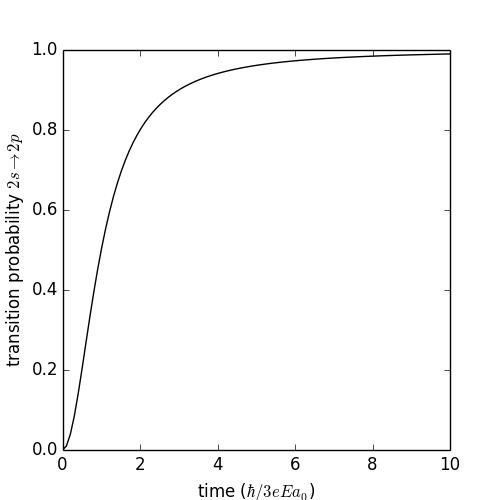
\includegraphics[width=0.65\textwidth]{transicion_stark.png}
\caption{\label{fig:transicion}Se muestra la probabilidad de transición del nivel $2s$ al nivel $2p$ en función del tiempo.}
\end{figure}

\end{enumerate}

\item

\begin{enumerate}[a)]

\item Bajo una transformación local con grupo de estructura $\textrm{U}(1)$ se tienen las transformaciones
\begin{align}
\begin{split}
\phi&\mapsto e^{-ig\theta}\phi,\\
A_\mu&\mapsto A_\mu-\partial_\mu\theta.
\end{split}
\end{align}
Estas a su vez inducen transformaciones sobre otros campos del Lagrangiano
\begin{align}
\begin{split}
\phi^*&\mapsto\qty(e^{-ig\theta}\phi)^*=e^{ig\theta}\phi^*,\\
\partial_\mu\phi&\mapsto\partial_\mu\qty(e^{-ig\theta}\phi)=e^{-ig\theta}\partial_\mu\phi-ige^{-ig\theta}\phi\partial_\mu\theta,\\
\partial_\mu A_\nu&\mapsto \partial_\mu(A_\nu-\partial_\nu\theta)=\partial_\mu A_\nu-\partial_\mu\partial_\nu\theta.
\end{split}
\end{align}
En primer lugar, se nota que
\begin{equation}
\phi^*\phi\mapsto e^{ig\theta}\phi^*e^{-ig\theta}\phi=\phi^*\phi.
\end{equation}
Esto concluye que el termino $-m^2\phi^*\phi$ es invariante. Por otra parte
\begin{equation}
F_{\mu\nu}\mapsto\partial_\mu A_\nu-\partial_\mu\partial_\nu\theta-\partial_\nu A_\mu-\partial_\nu\partial_\mu\theta=\partial_\mu A_\nu-\partial_\nu A_\mu=F_{\mu\nu}
\end{equation}
ya que las derivadas parciales conmutan\footnote{Esto no es cierto. Necesitamos asumir que $\theta$ es al menos $\mathcal{C}^2$. Esto no es problema ya que el grupo gauge se construye a partir de funciones $\mathcal{C}^\infty$.}. La invarianza del tensor electromagnético garantiza entonces la del termino de Maxwell $-\frac{1}{4}F_{\mu\nu}F^{\mu\nu}$. Finalmente,
\begin{align}
\begin{split}
\mathcal{D}_\mu\phi&\mapsto(\partial_\mu-ig(A_\mu-\partial_\mu\theta))\qty(e^{-ig\theta}\phi)\\
=&e^{-ig\theta}\partial_\mu\phi-ige^{-ig\theta}\phi\partial_\mu\theta-ige^{-ig\theta}A_\mu\phi+ige^{-ig\theta}\phi\partial_\mu\theta\\
=&e^{-ig\theta}\qty(\partial_\mu\phi-igA_\mu\phi)=e^{-ig\theta}\mathcal{D}_\mu\phi.
\end{split}
\end{align}
Conjugando obtenemos
\begin{equation}
(\mathcal{D}_\mu\phi)^*\mapsto e^{ig\theta}(\mathcal{D}_\mu\phi)^*
\end{equation}
lo que indica que
\begin{equation}
(\mathcal{D}_\mu\phi)^*(\mathcal{D}^\mu\phi)\mapsto e^{ig\theta}(\mathcal{D}_\mu\phi)^*e^{-ig\theta}\mathcal{D}^\mu\phi=(\mathcal{D}_\mu\phi)^*(\mathcal{D}^\mu\phi).
\end{equation}
Concluimos entonces que el término $(\mathcal{D}_\mu\phi)^*(\mathcal{D}^\mu\phi)$ es invariante y por lo tanto que el Lagrangiano lo es.

\item Calculamos las derivadas
\begin{align}
\begin{split}
\pdv{\mathcal{L}}{(\partial_\mu\phi^*)}=&\pdv{((\mathcal{D}_\nu\phi)^*\mathcal{D}^\nu\phi)}{(\partial_\mu\phi^*)}=\pdv{(\mathcal{D}_\nu\phi)^*}{(\partial_\mu\phi^*)}\mathcal{D}^\nu\phi=\pdv{(\partial_\nu\phi^*)}{(\partial_\mu\phi^*)}\mathcal{D}^\nu\phi\\
=&\delta_\nu^\mu\mathcal{D}^\nu\phi=\mathcal{D}^\mu\phi,\\
\pdv{\mathcal{L}}{\phi^*}=&\pdv{((\mathcal{D}_\mu\phi)^*\mathcal{D}^\mu\phi)}{\phi^*}-m^2\phi=\pdv{(\mathcal{D}_\mu\phi)^*}{\phi^*}\mathcal{D}^\mu\phi-m^2\phi\\
=&-igA_\mu\mathcal{D}^\mu\phi-m^2\phi.
\end{split}
\end{align}
Por lo tanto, las ecuaciones de Euler-Lagrange asociadas a $\phi$ se reducen a 
\begin{align}
\begin{split}
0=&\partial_\mu\pdv{\mathcal{L}}{(\partial_\mu\phi^*)}-\pdv{\mathcal{L}}{\phi^*}=\partial_\mu\mathcal{D}^\mu\phi+igA_\mu\mathcal{D}^\mu\phi+m^2\phi\\
=&(\partial_\mu+igA_\mu)\mathcal{D}^\mu\phi+m^2\phi=\mathcal{D}_\mu\mathcal{D}^\mu\phi+m^2\phi=\qty(\mathcal{D}_\mu\mathcal{D}^\mu+m^2)\phi.
\end{split}
\end{align}
Esta es precisamente la ecuación de Klein-Gordon al realizar el reemplazo $\partial_\mu\mapsto\mathcal{D}_\mu$.

\end{enumerate}

\item En vista de que
\begin{equation}
\pdv{F_{\sigma\rho}}{(\partial_\mu A_\nu)}=\pdv{(\partial_\sigma A_\rho-\partial_\rho A_\sigma)}{(\partial_\mu A_\nu)}=\delta_\sigma^\mu\delta_\rho^\nu-\delta_\rho^\mu\delta_\sigma^\nu,
\end{equation}
tenemos las derivadas
\begin{align}
\begin{split}
\pdv{\mathcal{L}}{(\partial_\mu A_\nu)}=&-\frac{1}{4}\pdv{(F_{\sigma\rho}F^{\sigma\rho)}}{(\partial_\mu A_\nu)}=-\frac{1}{4}F_{\sigma\rho}\pdv{F^{\sigma\rho}}{(\partial_\mu A_\nu)}-\frac{1}{4}\pdv{F_{\sigma\rho}}{(\partial_\mu A_\nu)}F^{\sigma\rho}\\
=&-\frac{1}{2}\pdv{F_{\sigma\rho}}{\partial_\mu A_\nu}F^{\sigma\rho}=-\frac{1}{2}(\delta_\sigma^\mu\delta_\rho^\nu-\delta_\rho^\mu\delta_\sigma^\nu)F^{\sigma\rho}=-\frac{1}{2}(F^{\mu\nu}-F^{\nu\mu})\\
=&-F^{\mu\nu},\\
\pdv{\mathcal{L}}{A_\nu}=&\frac{m^2}{2}\pdv{(A_\mu A^\mu)}{A_\nu}=\frac{m^2}{2}2A^\nu=m^2 A^\nu.
\end{split}
\end{align}
Por lo tanto las ecuaciones de Euler-Lagrange toman la forma
\begin{align}\label{ec:euler_lagrange_A}
\begin{split}
0=&\partial_\mu\pdv{F_{\sigma\rho}}{(\partial_\mu A_\nu)}-\pdv{\mathcal{L}}{(\partial_\mu A_\nu)}=-\partial_\mu F^{\mu\nu}-m^2 A^\nu\\
=&-\partial_\mu\partial^\mu A^\nu+\partial_\mu\partial^\nu A^\mu-m^2 A^\nu=-\qty(\partial_\mu\partial^\mu+m^2)A^\nu+\partial_\mu\partial^\nu A^\mu\\
=&-\qty(\Box+m^2)A^\nu+\partial^\mu\partial^\nu A^\mu=-g^{\nu\mu}\qty(\Box+m^2)A_\mu+\partial^\nu\partial^\mu A_\mu\\
=&-\qty(g^{\nu\mu}\qty(\Box+m^2)-\partial^\nu\partial^\mu)A_\mu.
\end{split}
\end{align}
Multiplicando por $-1$ y intercambiando los indices $\mu\leftrightarrow\nu$ se obtiene
\begin{equation}\label{ec:solucion_5}
0=\qty(g^{\mu\nu}\qty(\Box+m^2)-\partial^\mu\partial^\nu)A_\nu.
\end{equation}
Al tomar $\partial_\nu$ sobre la segunda linea de \eqref{ec:euler_lagrange_A} todos los indices se vuelven mudos y 
\begin{align}
\begin{split}
0=&-\partial_\mu\partial^\mu\partial_\nu A^\nu+\partial_\nu\partial^\nu\partial_\mu A^\mu-m^2\partial_\nu A^\nu\\
=&-\partial_\mu\partial^\mu\partial_\nu A^\nu+\partial_\mu\partial^\mu\partial_\nu A^\nu-m^2\partial_\nu A^\nu=-m^2\partial_\nu A^\nu.
\end{split}
\end{align}
Por lo tanto, si $m\neq 0$ se concluye que
\begin{equation}
0=\partial_\mu A^\mu.
\end{equation}
Note que en tal caso el termino $\partial^\nu A_\nu=\partial_\nu A^\nu=0$ de la ecuación \eqref{ec:solucion_5}. Por lo tanto se recupera la ecuación de Klein-Gordon
\begin{equation}
0=\qty(\Box+m^2)A^\mu.
\end{equation}

\end{enumerate}

\end{document}